\section{Results}
\label{sec:res}

\subsection{Discriminative threshold metrics of evaluation}
%
\Section{subsubsec:metricroc} and  \Section{subsubsec:metricpr} discuss methods that
Bauer et al.\ \cite{bauer2012bayesian} use to evaluate their model; these metrics are related to counting 
true- / false-positive / negative cases and varying a discriminative threshold.

\subsubsection{ROC curve}
\label{subsubsec:metricroc}
%
A receiver operating characteristic (ROC) curve requires a variable {\it threshold value} that specifies
the true- / false-positive / negative counts.
%
The threshold value that we use is rank.
%
More specifically,
all test items at or above rank $r$ are treated as positives, and the rest as negatives, 
where $r$ is the threshold variable.
%
Therefore, the $(0, 0)$ classifier is the classifier with a threshold of rank zero
(i.e., no ranked items are positives).
%
Similarly,  the $(1, 1)$ classifier is the classifier with a threshold rank of the
number of test examples (i.e., all ranked items are positives).

We plot ROC curves for 
all models, evaluated on the artificial patient data,
aggregating all diseases (\Figure{fig:rocartgen}),
on the artificial patient data,
for only the negatively annotated diseases
(\Figure{fig:rocartneg}), and for the naturalistic patient data,
aggregating all diseases (\Figure{fig:rocnatgen}).

\begin{figure}[!h]
    \begin{subfigure}{0.4\textwidth} \centering
    \begin{tikzpicture}[scale=0.85]
        \begin{axis}[legend pos=south east]
            \addplot table [x=fall-out, y=recall, col sep=comma]
            {analysis/generated_patients_all_no_freq_res_ROC.analysis};
            \addlegendentry{no freq}

            \addplot table [x=fall-out, y=recall, col sep=comma]
            {analysis/generated_patients_all_k_res_ROC.analysis};
            \addlegendentry{$k$-least freq}
            
            \addplot table [x=fall-out, y=recall, col sep=comma]
            {analysis/generated_patients_all_sampling_res_ROC.analysis};
            \addlegendentry{sampling}
            
            \addplot table [x=fall-out, y=recall, col sep=comma]
            {analysis/generated_patients_all_p_sampling_res_ROC.analysis};
            \addlegendentry{$p$-sampling}

            \addplot table [x=fall-out, y=recall, col sep=comma]
            {analysis/generated_patients_all_ic_res_ROC.analysis};
            \addlegendentry{IC-sampling}
        \end{axis}
    \end{tikzpicture}
    \caption{Artificial patient data; general disease.}
    \label{fig:rocartgen}
    \end{subfigure}
    \hfill
    \begin{subfigure}{0.4\textwidth} \centering
    \begin{tikzpicture}[scale=0.85]
        \begin{axis}[legend pos=south east]
            \addplot table [x=fall-out, y=recall, col sep=comma]
            {analysis/generated_patients_neg_no_freq_res_ROC.analysis};
            \addlegendentry{no freq}

            \addplot table [x=fall-out, y=recall, col sep=comma]
            {analysis/generated_patients_neg_k_res_ROC.analysis};
            \addlegendentry{$k$-least freq}
            
            \addplot table [x=fall-out, y=recall, col sep=comma]
            {analysis/generated_patients_neg_sampling_res_ROC.analysis};
            \addlegendentry{sampling}
            
            \addplot table [x=fall-out, y=recall, col sep=comma]
            {analysis/generated_patients_neg_p_sampling_res_ROC.analysis};
            \addlegendentry{$p$-sampling}
            
            \addplot table [x=fall-out, y=recall, col sep=comma]
            {analysis/generated_patients_neg_ic_res_ROC.analysis};
            \addlegendentry{IC-sampling}
        \end{axis}
    \end{tikzpicture}
    \caption{Artificial patient data; negatively-annotated disease.}
    \label{fig:rocartneg}
    \end{subfigure}

    \begin{center}
    \begin{subfigure}{0.4\textwidth}
    \begin{tikzpicture}[scale=0.85]
        \begin{axis}[legend pos=south east]
            \addplot table [x=fall-out, y=recall, col sep=comma]
            {analysis/phenotips_no_freq_res_ROC.analysis};
            \addlegendentry{no freq}

            \addplot table [x=fall-out, y=recall, col sep=comma]
            {analysis/phenotips_k_res_ROC.analysis};
            \addlegendentry{$k$-least freq}
            
            \addplot table [x=fall-out, y=recall, col sep=comma]
            {analysis/phenotips_sampling_res_ROC.analysis};
            \addlegendentry{sampling}
            
            \addplot table [x=fall-out, y=recall, col sep=comma]
            {analysis/phenotips_p_sampling_res_ROC.analysis};
            \addlegendentry{$p$-sampling}

            \addplot table [x=fall-out, y=recall, col sep=comma]
            {analysis/phenotips_ic_res_ROC.analysis};
            \addlegendentry{IC-sampling}
        \end{axis}
    \end{tikzpicture}
    \caption{Naturalistic patient data; general disease.}
    \label{fig:rocnatgen}
    \end{subfigure}
    \end{center}
    \caption{Receiver operating characteristic (ROC) curves.}
    \label{fig:roc}
\end{figure}

From the results in \Figure{fig:roc}, we see that all models performed almost equally well
according to the ROC metric, for both naturalistic and artificial data, and for general
diseases as well as negatively annotated diseases in particular.
%
However, while we see that the $p$-sampling and IC-sensitive $p$-sampling models
perform better than the other models on the pooled diseases (\Figure{fig:rocartgen}),
they perform worse on the negatively-annotated diseases (\Figure{fig:rocartneg}).
%
It is difficult to tell apart performance on the naturalistic data (\Figure{fig:rocnatgen}).


\subsubsection{Precision / recall curve}
\label{subsubsec:metricpr}
%
We plot precision-recall (PR) curves for 
all models, evaluated on the artificial patient data,
aggregating all diseases (\Figure{fig:prartgen}),
on the artificial patient data,
for only the negatively annotated diseases
(\Figure{fig:prartneg}), and for the naturalistic patient data,
aggregating all diseases (\Figure{fig:prnatgen}).
%
The PR curves also require definition of a threshold value $r$; we defined it
as described in \Section{subsubsec:metricroc}.
%
\begin{figure}[h]
    \begin{subfigure}{0.4\textwidth} \centering
    \begin{tikzpicture}[scale=0.85]
        \begin{axis}
            \addplot table [y=precision, x=recall, col sep=comma]
            {analysis/generated_patients_all_no_freq_res_PR.analysis};
            \addlegendentry{no freq}

            \addplot table [y=precision, x=recall, col sep=comma]
            {analysis/generated_patients_all_k_res_PR.analysis};
            \addlegendentry{$k$-least freq}
            
            \addplot table [y=precision, x=recall, col sep=comma]
            {analysis/generated_patients_all_sampling_res_PR.analysis};
            \addlegendentry{sampling}
            
            \addplot table [y=precision, x=recall, col sep=comma]
            {analysis/generated_patients_all_p_sampling_res_PR.analysis};
            \addlegendentry{$p$-sampling}
            
            \addplot table [y=precision, x=recall, col sep=comma]
            {analysis/generated_patients_all_ic_res_PR.analysis};
            \addlegendentry{IC-sampling}
        \end{axis}
    \end{tikzpicture}
    \caption{Artificial patient data; general disease.}
    \label{fig:prartgen}
    \end{subfigure}
    \hfill
    \begin{subfigure}{0.4\textwidth} \centering
    \begin{tikzpicture}[scale=0.85]
        \begin{axis}
            \addplot table [y=precision, x=recall, col sep=comma]
            {analysis/generated_patients_neg_no_freq_res_PR.analysis};
            \addlegendentry{no freq}

            \addplot table [y=precision, x=recall, col sep=comma]
            {analysis/generated_patients_neg_k_res_PR.analysis};
            \addlegendentry{$k$-least freq}
            
            \addplot table [y=precision, x=recall, col sep=comma]
            {analysis/generated_patients_neg_sampling_res_PR.analysis};
            \addlegendentry{sampling}
            
            \addplot table [y=precision, x=recall, col sep=comma]
            {analysis/generated_patients_neg_p_sampling_res_PR.analysis};
            \addlegendentry{$p$-sampling}
            
            \addplot table [y=precision, x=recall, col sep=comma]
            {analysis/generated_patients_neg_ic_res_PR.analysis};
            \addlegendentry{IC-sampling}
        \end{axis}
    \end{tikzpicture}
    \caption{Artificial patient data; negatively-annotated disease.}
    \label{fig:prartneg}
    \end{subfigure}
    
    \begin{center}
    \begin{subfigure}{0.4\textwidth} \centering
    \begin{tikzpicture}[scale=0.85]
        \begin{axis}
            \addplot table [y=precision, x=recall, col sep=comma]
            {analysis/phenotips_no_freq_res_PR.analysis};
            \addlegendentry{no freq}

            \addplot table [y=precision, x=recall, col sep=comma]
            {analysis/phenotips_k_res_PR.analysis};
            \addlegendentry{$k$-least freq}
            
            \addplot table [y=precision, x=recall, col sep=comma]
            {analysis/phenotips_sampling_res_PR.analysis};
            \addlegendentry{sampling}
            
            \addplot table [y=precision, x=recall, col sep=comma]
            {analysis/phenotips_p_sampling_res_PR.analysis};
            \addlegendentry{$p$-sampling}
            
            \addplot table [y=precision, x=recall, col sep=comma]
            {analysis/phenotips_ic_res_PR.analysis};
            \addlegendentry{IC-sampling}
        \end{axis}
    \end{tikzpicture}
    \caption{Naturalistic patient data; general disease.}
    \label{fig:prnatgen}
    \end{subfigure}
    \end{center}
    \caption{Precision-recall (PR) curves.}
    \label{fig:pr}
\end{figure}

The trend is clear for artificial patients from the results in \Figure{fig:prartgen} and \Figure{fig:prartneg}:
the IC-sensitive $p$-sampling model performs worst, with the $p$-sampling model 
performing next best; both are worse than the benchmarks.
%
However, we see that the sampling model is consistently better than the benchmarks.

Once again, the performance of different models on the naturalistic patient data
is hard to distinguish in \Figure{fig:prnatgen}.

\subsection{Other metrics of evaluation}
%
\Section{subsubsec:metricroc} and  \Section{subsubsec:metricpr} describe metrics
that are sensitive to the false positive count.
%
However, the way that we defined our threshold variable (rank) means that there are a
large number of false positives.
%
As well, our model is not a binary classifier in the strict sense, which ROC and PR curve
evaluation metrics expect; instead it is a ranking system.
%
Therefore, it seems necessary to evaluate our model by other metrics.
%
\Section{subsubsec:metricmrr} and  \Section{subsubsec:metricbrc} discuss methods that
rely on things other than the true- / false-positive / negative counts for evaluation.

\subsubsection{Mean reciprocal rank}
\label{subsubsec:metricmrr}

Define the {\it mean reciprocal rank} metric by the following computation:
%
\begin{align*}
    \text{mean reciprocal rank}
    &= \frac{1}{|S|} \sum_{k=1}^{|S|} \frac{1}{\text{rank}_k},
\end{align*}
where $S$ is the set of test cases, and rank$_k$ is the rank of the gold-standard 
disease in the $k$\textsuperscript{th} test case.
%
Then a large value of the mean reciprocal rank is indicative of good performance.

\begin{figure}[h]
    \begin{subfigure}{0.99\textwidth} \centering
    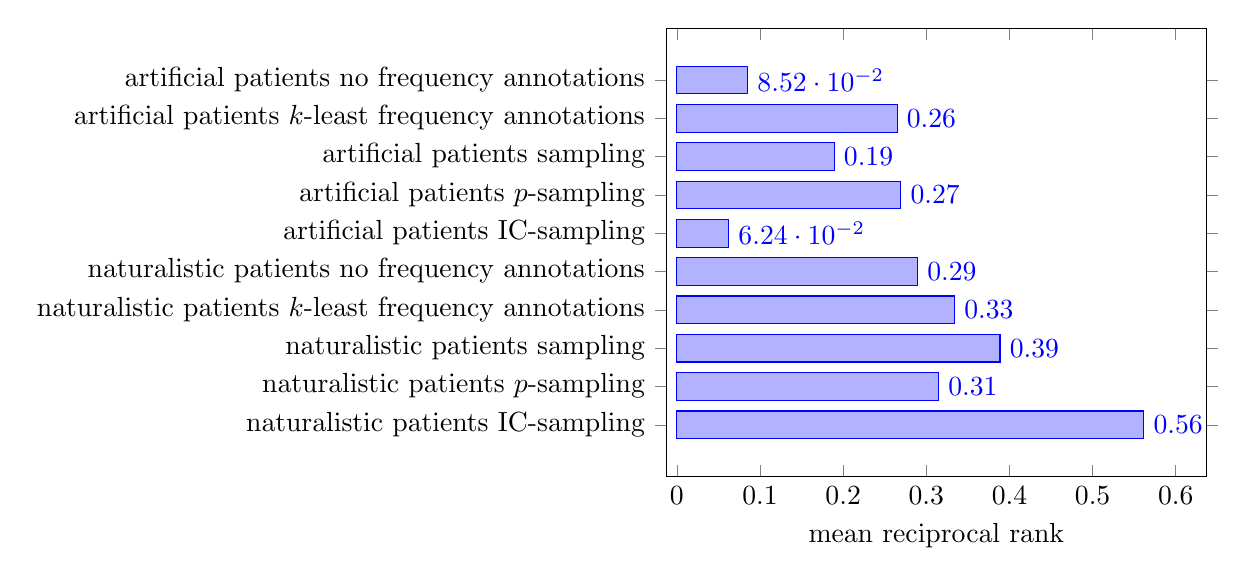
\begin{tikzpicture}
        \begin{axis}[
            xbar,
            enlargelimits=0.15,
            xlabel={mean reciprocal rank},
            symbolic y coords={
                % UPSIDE DOWN!
                naturalistic patients IC-sampling,
                naturalistic patients $p$-sampling,
                naturalistic patients sampling,
                naturalistic patients $k$-least frequency annotations,
                naturalistic patients no frequency annotations,
                artificial patients IC-sampling,
                artificial patients $p$-sampling,
                artificial patients sampling,
                artificial patients $k$-least frequency annotations,
                artificial patients no frequency annotations,
            },
            ytick=data,
            nodes near coords, 
            nodes near coords align={horizontal},
            yticklabel style={text height=1.5ex}, % To make sure the text labels are nicely aligned
            ]
            \addplot coordinates{
                (0.0852059148701,artificial patients no frequency annotations)
                (0.264807383628,artificial patients $k$-least frequency annotations)
                (0.189174526493,artificial patients sampling)
                (0.269227574751,artificial patients $p$-sampling)
                (0.062358752126,artificial patients IC-sampling)
                (0.289438943894,naturalistic patients no frequency annotations)
                (0.333880427171,naturalistic patients $k$-least frequency annotations)
                (0.388596491228,naturalistic patients sampling)
                (0.314673913043,naturalistic patients $p$-sampling)
                (0.561606160616,naturalistic patients IC-sampling)
            };
        \end{axis}
    \end{tikzpicture}
    \label{fig:mrrgen}
    \caption{All diseases pooled.}
    \end{subfigure}
    
    \vspace{1cm}

    \begin{subfigure}{0.99\textwidth} \centering
    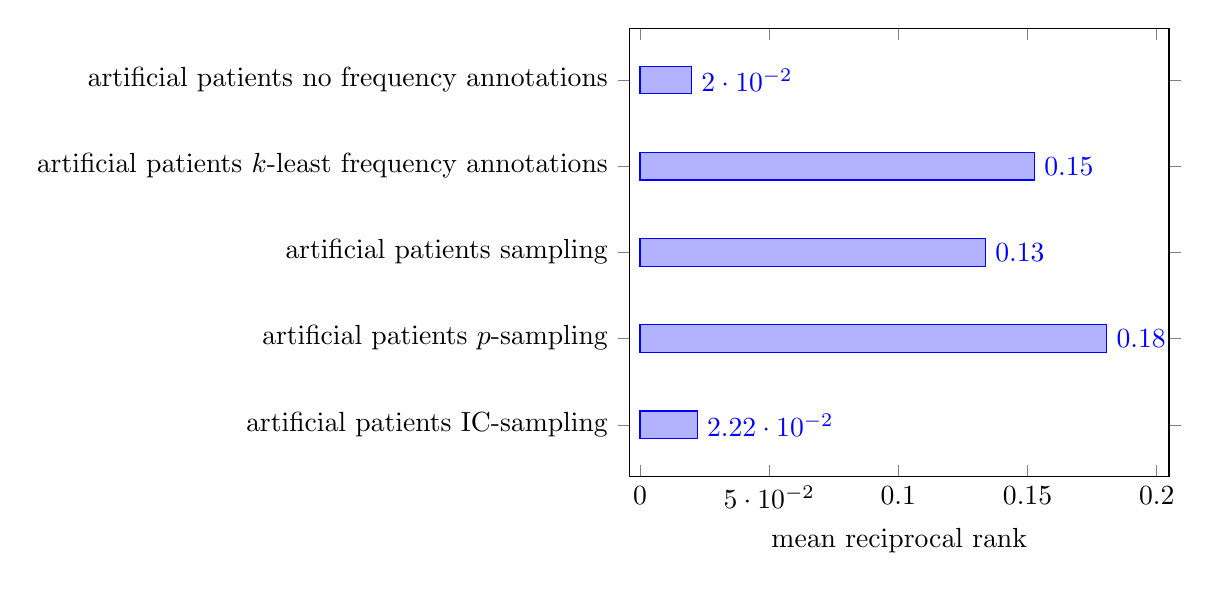
\begin{tikzpicture}
        \begin{axis}[
            xbar,
            enlargelimits=0.15,
            xlabel={mean reciprocal rank},
            symbolic y coords={
                % UPSIDE DOWN!
                artificial patients IC-sampling,
                artificial patients $p$-sampling,
                artificial patients sampling,
                artificial patients $k$-least frequency annotations,
                artificial patients no frequency annotations,
            },
            ytick=data,
            nodes near coords, 
            nodes near coords align={horizontal},
            yticklabel style={text height=1.5ex}, % To make sure the text labels are nicely aligned
            ]
            \addplot coordinates{
                (0.020012015728,artificial patients no frequency annotations)
                (0.152694351749,artificial patients $k$-least frequency annotations)
                (0.133770278138,artificial patients sampling)
                (0.180666666667,artificial patients $p$-sampling)
                (0.0221883556896,artificial patients IC-sampling)
            };
        \end{axis}
    \end{tikzpicture}
    \caption{Only diseases with negative annotations.}
    \label{fig:mrrneg}
    \end{subfigure}
    \caption{Mean reciprocal rank plots.}
    \label{fig:mrr}
\end{figure}

From the results in \Figure{fig:mrr}, we see an interesting pattern:
the models that perform relatively badly on the arificial data tend to perform well 
on the naturalistic data, according to this metric.
%
For example, the IC-sampling model performs worst on the artificial data, but performs
best on the naturalistic data.
%
The exception is the no-frequency model, which consistently performs badly, 
as to be expected because it is too simplistic.

\subsubsection{Binned rank counts}
\label{subsubsec:metricbrc}
%
To construct the binned rank plots,
we count the number of test cases for which the gold-standard disease falls into the
ranking bin of interest.

\begin{figure}[h]
    \begin{subfigure}{0.99\textwidth} \centering
    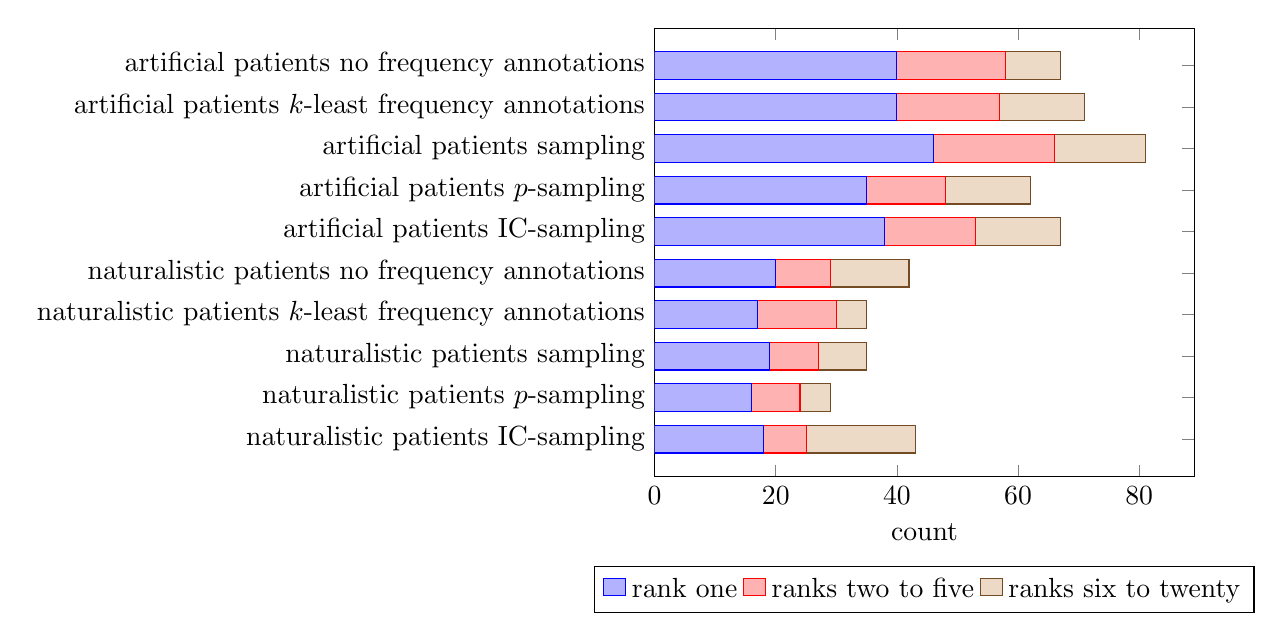
\begin{tikzpicture}
        \begin{axis}[
            xbar stacked,
            xlabel={count},
            xmin=0,
            legend style={at={(0.5,-0.20)}, anchor=north,legend columns=-1},
            symbolic y coords={
                % UPSIDE DOWN!
                naturalistic patients IC-sampling,
                naturalistic patients $p$-sampling,
                naturalistic patients sampling,
                naturalistic patients $k$-least frequency annotations,
                naturalistic patients no frequency annotations,
                artificial patients IC-sampling,
                artificial patients $p$-sampling,
                artificial patients sampling,
                artificial patients $k$-least frequency annotations,
                artificial patients no frequency annotations,
            },
            ytick=data,
            yticklabel style={text height=1.5ex}, % To make sure the text labels are nicely aligned
            ]
            \addplot coordinates{
                (40,artificial patients no frequency annotations)
                (40,artificial patients $k$-least frequency annotations)
                (46,artificial patients sampling)
                (35,artificial patients $p$-sampling)
                (38,artificial patients IC-sampling)
                (20,naturalistic patients no frequency annotations)
                (17,naturalistic patients $k$-least frequency annotations)
                (19,naturalistic patients sampling)
                (16,naturalistic patients $p$-sampling)
                (18,naturalistic patients IC-sampling)
            };
            \addlegendentry{rank one}
            \addplot coordinates{
                (18,artificial patients no frequency annotations)
                (17,artificial patients $k$-least frequency annotations)
                (20,artificial patients sampling)
                (13,artificial patients $p$-sampling)
                (15,artificial patients IC-sampling)
                (9 ,naturalistic patients no frequency annotations)
                (13,naturalistic patients $k$-least frequency annotations)
                (8 ,naturalistic patients sampling)
                (8 ,naturalistic patients $p$-sampling)
                (7 ,naturalistic patients IC-sampling)
            };
            \addlegendentry{ranks two to five}
            \addplot coordinates{
                (9 ,artificial patients no frequency annotations)
                (14,artificial patients $k$-least frequency annotations)
                (15,artificial patients sampling)
                (14,artificial patients $p$-sampling)
                (14,artificial patients IC-sampling)
                (13,naturalistic patients no frequency annotations)
                (5 ,naturalistic patients $k$-least frequency annotations)
                (8 ,naturalistic patients sampling)
                (5 ,naturalistic patients $p$-sampling)
                (18 ,naturalistic patients IC-sampling)
            };
            \addlegendentry{ranks six to twenty}
        \end{axis}
    \end{tikzpicture}
    \caption{Artificial and naturalistic patients; general disease.}
    \label{brc}
    \end{subfigure}
    
    \vspace{1cm}

    \begin{subfigure}{0.99\textwidth} \centering
    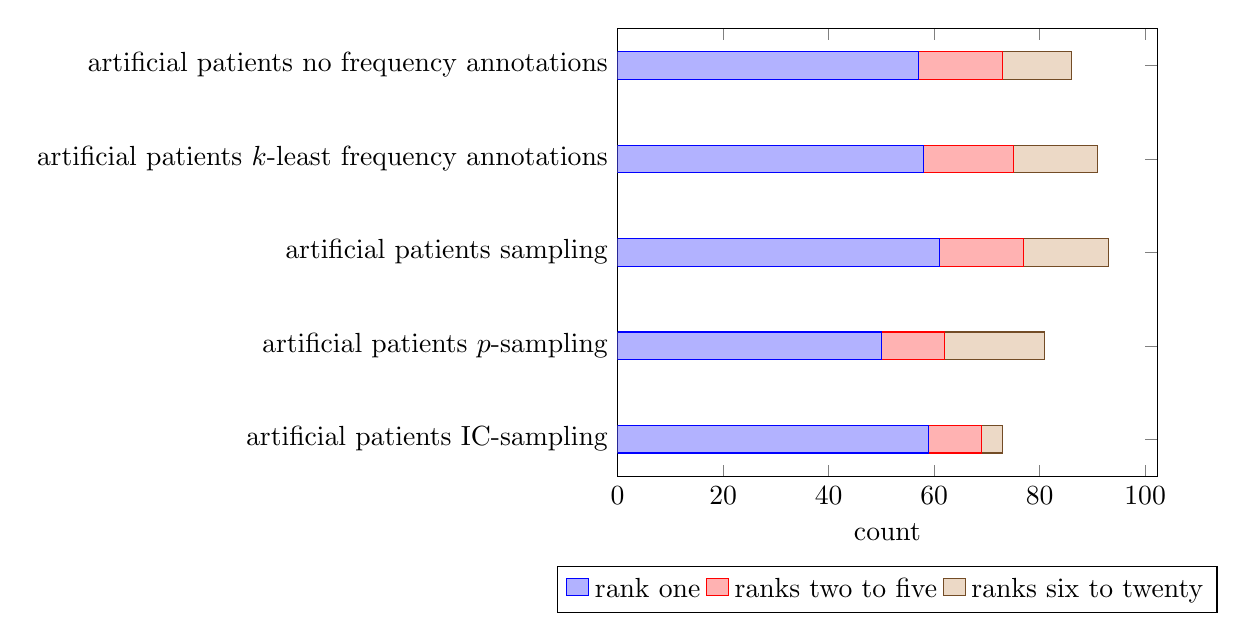
\begin{tikzpicture}
        \begin{axis}[
            xbar stacked,
            xlabel={count},
            xmin=0,
            legend style={at={(0.5,-0.20)}, anchor=north,legend columns=-1},
            symbolic y coords={
                % UPSIDE DOWN!
                artificial patients IC-sampling,
                artificial patients $p$-sampling,
                artificial patients sampling,
                artificial patients $k$-least frequency annotations,
                artificial patients no frequency annotations,
            },
            ytick=data,
            yticklabel style={text height=1.5ex}, % To make sure the text labels are nicely aligned
            ]
            \addplot coordinates{
                (57,artificial patients no frequency annotations)
                (58,artificial patients $k$-least frequency annotations)
                (61,artificial patients sampling)
                (50,artificial patients $p$-sampling)
                (59,artificial patients IC-sampling)
            };
            \addlegendentry{rank one}
            \addplot coordinates{
                (16,artificial patients no frequency annotations)
                (17,artificial patients $k$-least frequency annotations)
                (16,artificial patients sampling)
                (12,artificial patients $p$-sampling)
                (10,artificial patients IC-sampling)
            };
            \addlegendentry{ranks two to five}
            \addplot coordinates{
                (13,artificial patients no frequency annotations)
                (16,artificial patients $k$-least frequency annotations)
                (16,artificial patients sampling)
                (19,artificial patients $p$-sampling)
                (4,artificial patients IC-sampling)
            };
            \addlegendentry{ranks six to twenty}
        \end{axis}
    \end{tikzpicture}
    \caption{Artificial patients; disease with negative annotations.}
    \label{brc1}
    \end{subfigure}
    \caption{Binned ranking plots.}
\end{figure}

The results in \Figure{brc1} and \Figure{brc} show a similar trend to those described in
\Section{subsubsec:metricmrr}: models that tend to do well on the artificial data, do worse
on the naturalistic data and vice versa.
%
In particular, the IC-sampling model does best by a large margin on the naturalistic data,
but has very low performance on the artificial data.
%
The exception to the analogy to
\Section{subsubsec:metricmrr} is that the sampling method performs well in both 
artificial and naturalistic data scenarios.
